\chapter{Background}

Related work and the state of the art were reviewed, and identification of
relevant background material was carried out in the project preceding this
thesis \cite{aven_exploring_2019}. This background is herein amended with
further insights into the paradigm of physical reservoir
computing. Specifically, the main focus is transferred from physical limitations
in general, to the narrower scope of spatial limitations relating to physical
morphology and topology.

\section{Order and Chaos}

A section on the main interesting points about order and chaos in the context of
reservoir computing could maybe serve as a gentle introduction of the underlying
principles?

I.e.: should a section be included that briefly explains the relevance of the
line of criticality? Perhaps illustrating the subject with the Lyapunov
exponent. The degree of sensitivity to initial conditions might not be
completely relevant, but the theory as a whole is important.

``Dynamic Systems and Computing at the Edge of Chaos''?

\section{Reservoir Computing}

``Instead it proposes that the trajectory of internal states of a recurrent
neural circuit provides a raw, unbiased, and universal source of temporally
integrated information, from which specific readout elements can extract
specific information about past inputs for their individual task.'' maass paper

\subsection{Recurrent Neural Networks}

Their use, and why backward edges makes it notoriously difficult to train such
networks.

Problems with RNN and LSTM: page 5 of ``Short Term Memory in ESNs'', by Jaeger
has some info on LSTM problem with chaos, and RNN training problem on long
temporal dependencies.

\subsection{Echo State Networks}

The inception of reservoir computing as a methodology with Jaeger's Echo State
Network and Maass's Liquid State Machine.

A section that specifically explains how the default Echo State Networks
function. Some minor details about work that has been done to improve upon the
model, such as intrinsic plasticity, leaking neurons, and so on.

``schrauwen_improving_2008''

Common tunings, such as input scaling, spectral radius, leakage and sparsity.

Extensions to base model. Bias, output feedback, teacher forced etc.

Echo State Property.

\subsection{Real World Applications}

Present some real world applications, like equalizing wireless communication
channel, short-term traffic load, short-term electric load, stock forecasting.

Robot navigation mentioned in model for-in materio by dale, also interesting
overall

Find the funny one about printers that break (lol)

some presented in pre-thesis

\subsection{Comparison to State of the Art}

Perhaps a short comparison to RNN training methods, LSTM, and GRU.

\section{Physical Reservoir Computing}

anything exhibiting complex dynamic behavior.

The emergence of physical substrates as a medium for the reservoir computing
paradigm. Illustrate some of the main topics, like photonics, optoeletronics,
mechanical (coupled oscillators), biologically inspired (ecoli, invitro),
magnetism. Use the survey paper.

It is importance to stress that we are considering alternatives to the
traditional reservoirs in this section. Drive home the point that we are
exploring physical mediums that are wildly different from traditional computers,
where memory and computation and fundamentally separate.

``Reservoir Computing as a Model for In-Materio Computing''

``Lattice networks/models are common in computational physics, condensed matter
physics and beyond, modelling physical interactions, phase transitions and
structure [15]. Examples include: discrete lattices like the Ising model with
variables representing magnetic dipole moments of atomic spins, and the Gray-
Scott reaction-diffusion model to simulate chemical systems [22]. Also, physical
substrates often have a regular grid of connections. Lattice networks are
therefore more realistic representations of many physical systems that would be
considered for reservoir computing.'' from role of structure and complexity

``There are many physical properties and considerations that require discussion
when talking about using any novel material for computation. Here we focus on four
key factors that possess some relevance to substrate-based reservoirs: (i) a means
by which to observe network connectivity and activity, (ii) assuring non-linearity is
present in the system, (iii) methods for modelling activity and behaviour, and (iv)
the impact of environmental factors.'' from in-materio paper dale.

\subsection{Spatial Networks}

Use a previous section on physical reservoir computing to lead into background
on networks that are manifested into a physical space. Talk about previous work,
such as the Minimum Complexity Echo State Network.

Discuss existing theory on spatial networks. Relevant topics may include the
Erdős–Rényi model as a basis for Echo State Networks, then the Waxman model with
its physical restraints, and then a dive further into completely regular
structures such as lattices.

\section{Assessing Reservoir Quality}

Designing \textit{good} reservoirs, possessing some set of desired properties,
naturally requires some metric by which we can evaluate and compare. Parameter
sweeps, i.e. our trial and error methods, must be accompanied by sufficient
methods of assessing computational performance.

Evaluation of reservoir quality is split into two different
approaches. Intuitively, measuring the performance of the model on a given
benchmark task is a simple, direct way of assessment. However, to gain an
intuition for a more general, expected performance across multiple benchmarks,
one may measure independent properties of the system, e.g. the spectral radius
of the internal weight matrix. The two approaches are often used in conjunction,
combined to propose an overall quality.

\subsection{Independent Metrics}

\subsubsection{Kernel Quality and Generalization}

Within the RC paradigm we are concerned with producing a complex mapping from
the input stream to some spatial, internal representation, such that a
memory-less, linear readout map may be employed for classification.

The \textit{linear separation property}, or \textit{kernel quality}, measures
ability to separate different inputs \cite{legenstein_edge_2007}. It is an
empirical measure of this complex mapping, denoting the potential diversity of
nonlinear operations carried out by a reservoir. Kernel quality is evaluated by
presenting a reservoir of size $n$ with $m$ different input sequences, and
computing the rank of the resulting $m\times n$ matrix consisting of the
reservoir states resulting at some time step $t$ for the input stream
\cite{busing_connectivity_2010}.

Another metric accompanying the kernel quality is the \textit{generalization
capability} of the reservoir \cite{legenstein_edge_2007}. This metric addresses
ability to generalize already learned functions or filters to new, unseen input,
and is used as an estimation of the VC-dimension of the
reservoir. Generalization capability is evaluated with the same method as kernel
quality, but instead requires input streams that are similar, or belong to the
same class \cite{busing_connectivity_2010}.

A reservoir in the ordered regime will naturally exhibit low values on both
metrics, while both metrics will be high in a network in the chaotic
regime. Thus, in general, reservoirs exhibiting a high kernel quality and a low
generalization rank are desirable, and the difference between the two is
sometimes used as its own metric \cite{busing_connectivity_2010}.

\subsubsection{Short-Term Memory}

Short-term memory capacity was introduced as a quantitative measurement of
linear memory capacity in reservoirs \cite{jaeger_short_2002}. It is a way to
examine the fading memory present in the system, and is measured by attaching
output units to the reservoir, which each are trained to recall some time
delayed version of the input sequence. By measuring how much of the input each
output unit can recover, we can estimate the memory capacity $MC$ by summing
over all time delays. Jaeger defined this as

\begin{equation}
  MC =
  \sum_{k}^{\infty}MC_{k} =
  \frac
  {cov^2(u(t-k), y_k(t))}
  {\sigma^{2}(u(t))\sigma^{2}(y_{k}(t))}
  ,
  \label{stm-eq}
\end{equation}

where $MC$ in general is limited by the reservoir size $N$, such that $MC \leq
N$. High input retention is a desirable property, but an increase in memory
capacity through parameter tuning is often met with a decrease in complex
information processing, due to a universal trade-off between memory and
nonlinearity \cite{dambre_information_2012}.

% (TODO): Not entirely orthogonal from generalization (see Burkow).

% (TODO): Cite "Computational analysis of memory capacity in echo state
% networks" in the methodology section of this specifically for ESNs.

\subsubsection{Memory-Nonlinearity Trade-off}

Experimentation with a wide range of reservoirs has indicated a crucial
interplay between the memory and nonlinearity properties in reservoir operation
\cite{verstraeten_memory_2010}. In fact, the interplay has been uncovered to be
a universal trade-off between depth of memory and nonlinear computation
performed by a dynamical system \cite{dambre_information_2012}.

Thus, analyzing the boundary between an ordered, static regime that provides
memory, and a chaotic, dynamic regime that provides processing, is of vital
importance in the design of reservoirs. Determining the required nonlinearity
for a task is not a simple task, and often benefits from intuition about
nonlinear dynamics. Empirically, it has been shown that the input scaling,
determining the nonlinearity of reservoir responses, and the spectral radius,
scaling the importance of previous states, are the main parameters for
optimization in ESNs, illustrating the significance of the trade-off
\cite{montavon_practical_2012}.

Further formalization of the trade-off has been conducted, accompanied by a
proposition of a mixture reservoir combining both linear and nonlinear
dynamics. Adding a ``pinch of linearity'' is cited to improve performance
considerably \cite{inubushi_reservoir_2017}.

\subsubsection{Further Metrics}

Lots about this in ``Reservoir Computing as a Model for In-Materio Computing''.

Also shortly present alternative metrics that are sometimes used, such as
Lyapunov spectrum, Lyapunov exponent, separation ratio line thing etc.

We may go the opposite way of ESN: i.e. instead of scaling by spectral radius,
it is instead an actual property we can measure to predict performance.

``On the quantification of dynamics in Reservoir Computing''.

lyapunov exponent and kernel quality correlate ``On the correlation between
reservoir metrics and performance for time series classification under the
influence of synaptic plasticity.''

\subsection{Benchmarks}

Employing benchmarks to measure the performance of reservoirs is a means to
directly capture performance on specific tasks. Myriads of benchmarks exist
within the field of time series prediction, generation, and classification. The
benchmark spectrum range from simple tasks, to complicated, highly dynamic and
autoregressive time series.

Simpler tasks include the XOR problem of which is not linearly separable
\cite{goos_pattern_2003}, and n-bit temporal density and parity
\cite{bertschinger_real-time_2004}. More complex tasks may range from
recognizing isolated digits in speech \cite{verstraeten_isolated_2005}, to
predicting time series, of which the most popular are the Mackey-Glass time
delay differential equation \cite{mackey_oscillation_1977}, and the nonlinear
autoregressive moving average, NARMA \cite{atiya_new_2000}. Further datasets,
such as the Santa Fe Laser, Hénon Map, IPIX Radar, and Sunspot series datasets
have also been used \cite{rodan_minimum_2011}.

\subsubsection{NARMA - Nonlinear Autoregressive Moving Average}

\begin{figure}[t!]
  \centering
  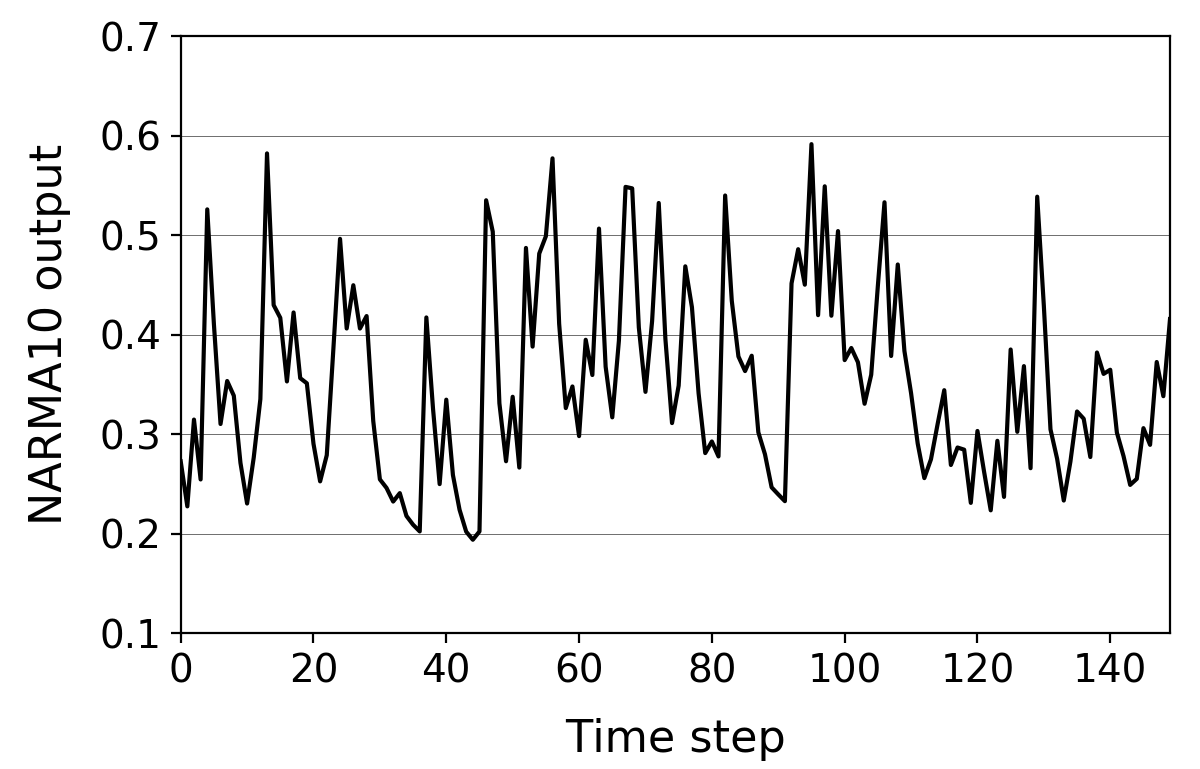
\includegraphics[width=3.0in]{figures/NARMA10.png}
  \caption{
    Example output generated by a 10th-order NARMA system. The autoregressive
moving average nature of the time series is clearly visible.
  }
  \label{narma10-fig}
\end{figure}

The class of time series provided by a nonlinear autoregressive moving average,
most often simply referred to as \textit{NARMA}, is a model commonly used to
benchmark recurrent networks \cite{atiya_new_2000}. Its widespread use yields
baseline performances for well established models, as well as more novel
approaches \cite{verstraeten_experimental_2007, appeltant_information_2011}.

NARMA provides discrete-time temporal tasks, introducing a time-lag of $n$ time
steps, and is given by

\begin{equation}
  y_{t} = \alpha y_{t-1} +
  \beta y_{t-1} \sum_{i=1}^{n}y_{t-i} +
  \gamma u_{t-1}u_{t-n} +
  \delta
  .
  \label{narma-eq}
\end{equation}

Here, $n$ is the order of the system, and common constant parameters are $\alpha
= 0.3$, $\beta = 0.05$, $\gamma = 1.5$ and $\delta = 0.1$. The input $u_{t}$ is
an i.i.d. stream drawn uniformly from the interval [0, 0.5]. The time series is
unstable, and tasks with higher than a 10th-order time lag introduce a
saturation function to produce a bounded sequence:

\begin{equation}
  y_{t} =
  \tanh(
  \alpha y_{t-1} +
  \beta y_{t-1} \sum_{i=1}^{n}y_{t-i} +
  \gamma u_{t-1}u_{t-n} +
  \delta
  )
  .
  \label{narma-tanh-eq}
\end{equation}

% (TODO): Perhaps plot nonlinearity of multiplying values in [0.0, 0.5]? See
% Verstraeten on memory-nonlinearity trade-off.

Predicting a NARMA time series, given an input sequence $u$, presents a
challenge of both memory and nonlinearity. This makes NARMA well-suited for
evaluating both the memory capacity and computational power of reservoirs with a
single metric. Reservoirs must necessarily remember input sequences of length
$n$, and should preferably adhere to suitable dynamics on top of this. A
10th-order system is depicted in Figure \ref{narma10-fig}

Evaluation of ESN performance on the NARMA10 system is a thoroughly explored
area in the field of RC. Reported NRMSE performances for traditional ESN
reservoirs of size $N = 200$ lie in the range [0.20, 0.25]
\cite{rodan_minimum_2011, verstraeten_experimental_2007,
goudarzi_comparative_2014, jaeger_adaptive_2003}. For some context, using a
shift register containing the input as a reservoir will achieve a minimal NRMSE
of 0.4. To achieve NRMSE values below this threshold it is necessary to
introduce nonlinearity in the reservoir.

%%% Local Variables:
%%% mode: latex
%%% TeX-master: "../thesis"
%%% End: